%====================================================================================================
% ?????
%====================================================================================================
% TCC
%----------------------------------------------------------------------------------------------------
% Autor				: Jasane Schio
% Orientador		: Gedson Faria
% Co-Orientador		: Angelo Darcy
% Instituição 		: UFMS - Universidade Federal do Mato Grosso do Sul
% Departamento		: CPCX - Sistema de Informação
%----------------------------------------------------------------------------------------------------
% Data de criação	: 01 de Outubro de 2015
%====================================================================================================

\chapter{Primeiros Resultados - Seleção Manual de Mínimos e Máximos}
 \label{Cap:Resultados}

Neste capítulo são apresentados os resultados dos testes realizados. 

A primeira etapa do projeto, já concluída, é a seleção manual de mínimos e máximos. Nessa etapa foi gerado uma imagem Threshold onde somente objetos que possuam seu HSV entre os valores calibrados apareçam. 
\begin{figure}[h]
	\centering
	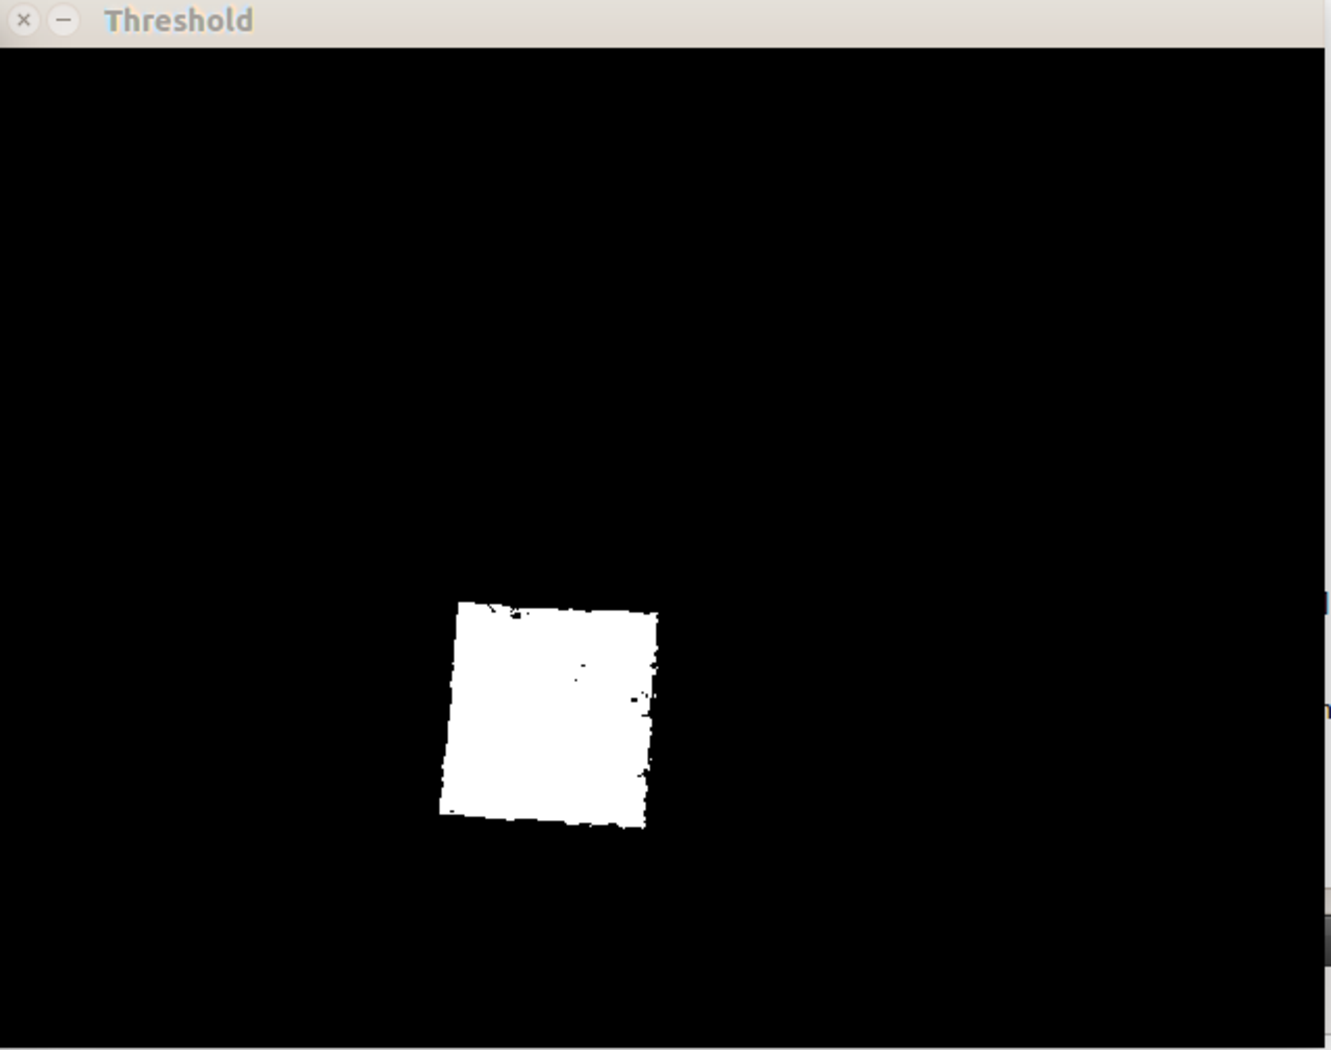
\includegraphics[width=0.8\textwidth]{resultado.pdf}
	\caption{Threshold gerado apos seleção manual.}
	\label{ResultadoManual}
\end{figure} 
%\section{Resultados Final -  Seleção Inteligente de Mínimos e Máximos} \label{Sec:Resultado1}

